\documentclass[11pt]{article}
\usepackage{graphicx}
\usepackage{geometry}
\usepackage{float}
\usepackage{amsmath}
\usepackage{circuitikz}
\usepackage{amssymb}
\usepackage{mathtools}
\usepackage{tikz}
\usepackage{tikz-3dplot}
\usepackage{cite}
\DeclarePairedDelimiter{\set}{\{}{\}}

\title{Counting Statistics}
\author{Spandan Suthar and Timo Peschken}
\date{October 28, 2025}

\geometry{margin=1in}
\setlength{\parindent}{0pt}

\begin{document}

\maketitle

\section{Introduction}

Radioactive materials emit a collection of particles. Using a
scintillation detector and a single channel analyzer, the number of particles
emitted by a particular radioactive sample within a single time
period can be measured. In this experiment, emissions of a
radioactive sample are counted over a number of trials for two time periods:
a long ("high count") time period and a short ("low count") time
period. The resulting data are analyzed using high and low count
statistics---using a Gaussian distribution and a Poisson distribution---and the
counts are found to agree well with the theoretical predictions of
either distribution.

\section{High Count Statistics}

\begin{figure}[H]
  \centering
  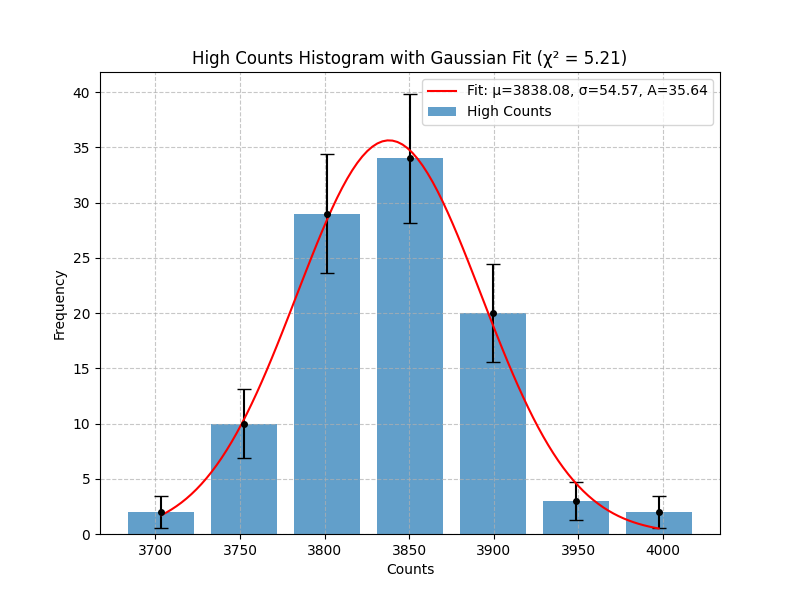
\includegraphics[width=0.8\textwidth]{../high_counts_histogram.png}
  \caption{Frequency of counts vs. binned emission counts for
    long-time, large-count trials, in blue. Error bars representing
    uncertainties in bin counts are shown in black, while a Gaussian
  distribution fit to the data is shown in red.}
  \label{fig:high_counts_histogram}
\end{figure}

Binned frequencies of emission counts versus counts are shown in Figure
\ref{fig:high_counts_histogram}. A Gaussian distribution is fit
to the data to yield a chi-squared value of $\chi^2 = 5.21$,
comparable to the number of bins used, 7. Experimental values of $\hat \mu =
3838.08$ and $\hat \sigma = 35.64$ are obtained from fitting.
The fit Gaussian's cumulative coefficient (its standard normalization
  constant times the additional scaling factor necessary to fit the
dataset) is found to be $\hat A = 35.64$. A sample mean with standard
deviation of the mean is obtained
directly from the data: $\mu \pm \sigma_{\mu} = 3838 \pm 6$.

\vspace{1em}

The counts of the high count trial were obtained over a period of $T
= 10 \pm 0.01$ s. The average counting rate, using the best estimate
for the mean of counts and the standard deviation of the mean, is $R
= \frac{N}{T} = 38.38 \pm 0.07$ Hz. Note that the standard
deviation of the mean and not the standard deviation of the counts
is used; the former estimates the uncertainty in an input variable
to the average counting rate, while the latter estimates a more
pointwise uncertainty.

\vspace{1em}

% TODO: uncertainties on the counts

A count of values within
$1\sigma$ and $2\sigma$ of $\mu$ is also found, yielding proportions
of $0.73 \pm 0.09$ and $0.9 \pm 0.1$ relative to all 100 points.
(Note: $\mu$ is the sample mean and $\sigma$ is the sample standard
deviation). The Gaussian function fit to the data is numerically integrated to
estimate the same quantities, yielding $1\sigma$- and $2\sigma$-proportions of
$0.70 \pm 0.08$ and $1.0 \pm 0.10$, respectively.

\vspace{1em}

The sample mean and mean from fitting agree within 1$\sigma_{\mu}$ of
each other, while the proportions of counts within $1
\sigma$ and $2 \sigma$ of the sample mean agree within $1
\sigma_{p_1}$ and $1 \sigma_{p_2}$ of each other in both proportion
analyses (where $\sigma_{p_1}$ and $\sigma_{p_2}$ are the
uncertainties in the discrepancies between the corresponding proportions).

\section{Low Count Statistics}

\begin{figure}[H]
  \centering
  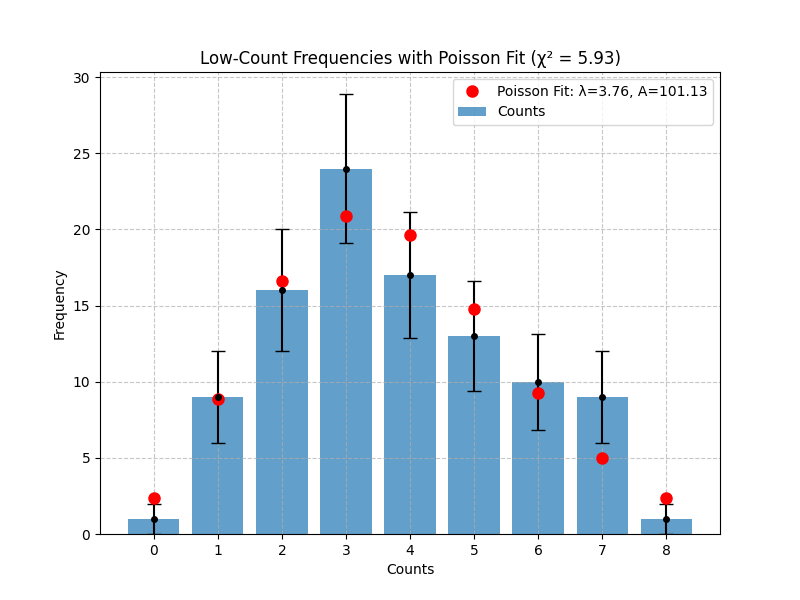
\includegraphics[width=0.8\textwidth]{../low_counts_histogram.png}
  \caption{Frequency of counts vs. binned emission counts for
    short-time, small-count trials, in blue. Error bars representing
    uncertainties in bin counts are shown in black, while a Poisson
  distribution fit to the data is shown in red.}
  \label{fig:low_counts_histogram}
\end{figure}

A similar binning analysis is performed for the low count data.
Fitting a Poisson distribution to the counts of each bin produces a
chi-squared value of $\chi^2 = 5.93$, comparable to the number of bins used, 9.
The resulting mean from the Poisson fit is $\lambda = 3.76$. Using
the standard deviation of the mean, the sample mean of counts
is found to be $\mu \pm \sigma_{\mu} = 3.77 \pm 0.18$.

\vspace{1em}

The sample mean and the mean from the Poisson fit agree within $1
\sigma_{\mu}$ of
each other, providing some evidence for a Poisson-distributed
dataset. However, the sample mean and sample variance $\sigma^2
\approx 3.33$ of the data are about $2.4\sigma_{\mu}$ apart,
suggesting the data is on the boundary of being Poisson distributed. An ideal
Poisson distribution would have a sample mean and sample variance
that are equal.

\section{Conclusion}

The distribution of high counts agrees well with a Gaussian
distribution. Analysis of the fit yields a chi-squared value of
$\chi^2 = 5.21$ for 7 bins, while the number of points falling within
$1\sigma$ and $2 \sigma$ of the mean agree with the theoretical values
of $0.68$ and $0.95$, respectively. This pattern continues for the low-count
analysis: a Poisson distribution fit to the data gives a chi-squared value of
$\chi^2 = 5.93$ for 9 bins, though the mean and variance are found to
be a large $2.4 \sigma$ apart. Both the Gaussian and Poisson
distributions' means are in excellent agreement with the
corresponding sample means.

\end{document}
